\chapter{Especificación de Requisitos}
\label{cap:EspecificaciondeRequisitos}
\title{Especificación de Requisitos}

Para lograr que el desarrollo de un sistema hardware o software sea un éxito,
es necesario que los desarrolladores comprendan totalmente las especificaciones que
requiere el proyecto. En esta sección se va a proceder a enumerar los requisitos del
sistema en el que se está trabajando.\\

\title{Modelado del sistema}
\section{
Modelado del sistema
}

El dispositivo que se desea desarrollar tiene que hacer la función básica
del director de la banda de música durante una actuación, es decir,
marcar el mismo pulso a los músicos.\\

Cuando la agrupación se encuentra realizando un concierto, el
esquema de comunicación que se sigue es el mostrado en la figura \ref{fig:modeladoconceptual}
(donde el nodo rojo es el director y lo morados los músicos). El único flujo de información
que hay es que que marcan las flechas (el pulso, que sigue un tempo constante). Hay que
aclarar que en este caso, para simplificar, sólo se han dibujado 5 músicos,
sin embargo, como se vio en la introducción, las bandas suelen contar entre sus filas con
varias decenas de integrantes.\\


\begin{figure}[htb]
\centering
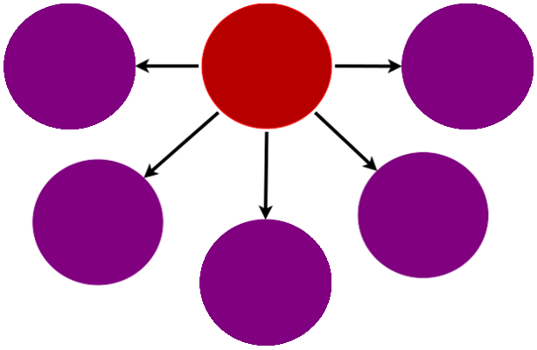
\includegraphics[width=0.6\textwidth]{./imagenes/modeladoconceptual}
\caption{Modelado del sistema} \label{fig:modeladoconceptual}
\end{figure}

El flujo de información es el mostrado en la figura \ref{fig:mensajesconceptual}
  \begin{figure}[htb]
  \centering
  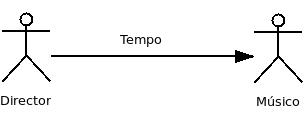
\includegraphics[width=0.6\textwidth]{./imagenes/mensajesconceptual}
  \caption{Traspaso de información} \label{fig:mensajesconceptual}
  \end{figure}


Es necesario guardar el ``tempo'' (que será establecido por el director) y algún tipo
de idenficación de los músicos, para que el director sepa con quién se tiene que
comunicar (aunque esto se verá más adelante).\\


\title{Actores}
\section{Actores}
\label{sec:actoresRequisitos}

Del esquema de la figura \ref{fig:mensajesconceptual} podemos sacar una conclusión clara:
será necesaria la distinción entre dos tipos de usuarios en nuestro sistema.
  \begin{itemize}
    \item Director: es el que envía el pulso al resto de actores. Solo uno por sistema
    \item Músico: recibe el pulso del director. Habrá multiples
  \end{itemize}


\title{Requisitos funcionales}
\section{Requisitos funcionales}

En este apartado se van a describir los requisitos funcionales del sistema.
Estos requisitos son aquellas funciones o capacidades que el sitema debe
tener para satisfacer las necesidades de los usuarios.\\

\begin{itemize}
    \item[\textbf{RF.1}] El sistema permitirá al director insertar un tempo
    \item[\textbf{RF.2}] Se capacitará al director para hacer llegar el pulso adecuado a los intérpretes
    \item[\textbf{RF.3}] El pulso se comunicará a los músicos a través de algún actuador (una señal visual, por ejemplo)
\end{itemize}


\title{Requisitos no funcionales}
\section{Requisitos no funcionales}

En estea sección se van a describir los distintos requisitos no funcionales del sistema.
Los requisitos no funcionales son aquellos que nos informan de restricciones que debe cumplir
nuestro sistema.\\


\begin{itemize}
    \item[\textbf{RNF.1}] El sistema debe ser wireless: la comunicación entre los
      dispositivos debe hacerse sin cables
    \item[\textbf{RNF.2}] Debe de ser barato: para que el usuario desee utilizar
      el sistema, este debe tener un coste asumible
    \item[\textbf{RNF.3}] La escalabilidad no debe ser un problema: se deben poder añadir
      muchos dispositivos al sistema y que la funcionalidad no se resienta.
    \item[\textbf{RNF.4}] Debe permitir que se puedan añadir funciones: para futuras mejoras.
    \item[\textbf{RNF.5}] El dispositivo que se desarrolle tiene que ser discreto y cómodo:
      ningún usuario va a querer utilizarlo si se siente mal llevándolo o si es demasiado llamativo.
    \item[\textbf{RNF.6}] Bajo consumo energético: se busca aprovechar la batería al máximo
      (si el dispositivo funciona durante poco tiempo, no habrá usuarios que deseen utilizarlo).
    \item[\textbf{RNF.7}] Sincronización entre los músicos: ya que lo que se busca es dar unidad
      a la interpretación de las distintas obras, el sistema debe cumplir unos requisitos de tiempo
      importantes (a nivel de milisegundos para que, en caso de haber algo de asincronía, el usuario no lo note).
    \item[\textbf{RNF.8}] El pulso debe mantenerse constante: el pulso, por definición
      no cambia a lo largo de la obra y debe conseguirse que el usuario lo perciba de forma
      constante
\end{itemize}


\title{Requisitos de información}
\section{Requisitos de información}

Estos requisitos indican qué información guarda nuestro sistema.\\

  \begin{itemize}
    \item[\textbf{RI.1}] Tempo: se guardará el tempo indicado por el director
    para poder transmitir el pulso adecuado a los distintos músicos o, en su defecto,
    enviar el tempo una vez que estén sincronizados
    \item[\textbf{RI.2}] Músicos: el director deberá conocer los músicos existentes en la banda
    para saber a quién tiene que comunicarle el tempo. Podría darse el caso de dos
    agrupaciones musicales que se encontrasen muy próximas y utilizase en sistema:
    hay que evitar que el pulso de una de las bandas interfiera el de la otra
  \end{itemize}
